\chapter{A starting point}
\lettrine[lines=4]{G}{raphs} do things and stuff.  They have recieved a great
deal of attention lately because they can model real world \textit{relationships}.  But what is
a graph?  

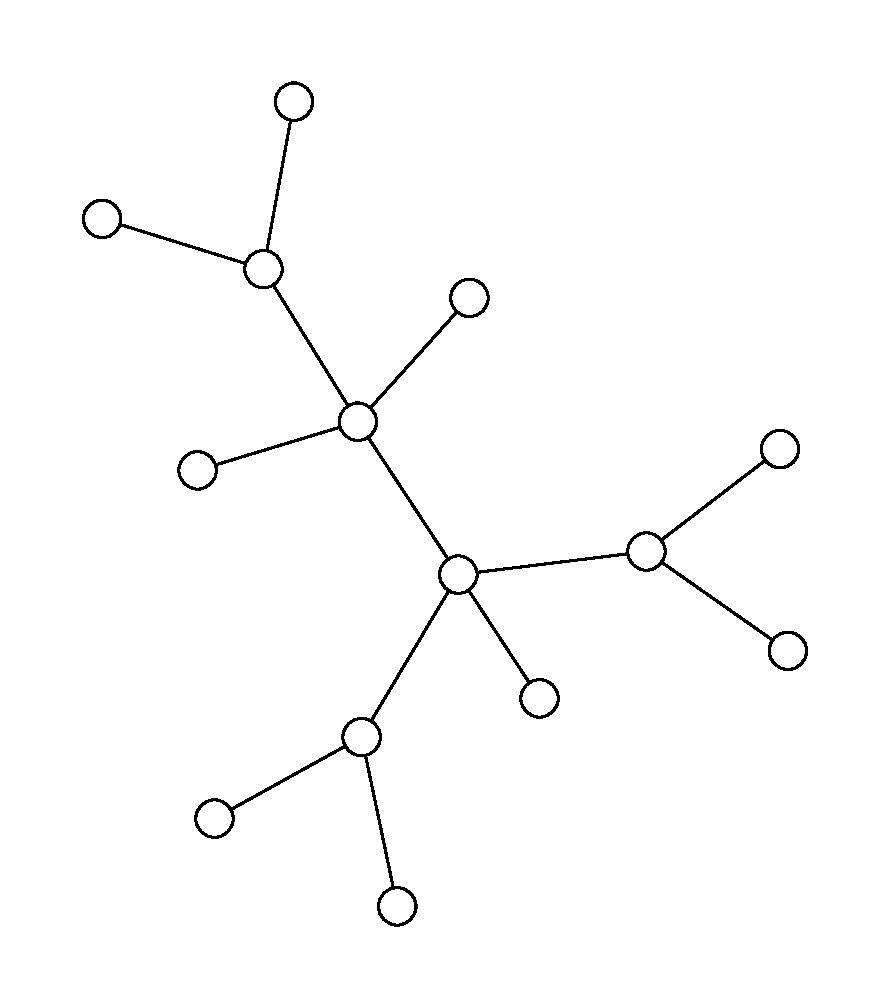
\includegraphics[width=0.4\textwidth]{tree.pdf}

\begin{figure}%
    \centering
    \subfloat[k5]{{\includegraphics[width=0.4\textwidth]{k5.pdf} }}%
    \qquad
    \subfloat[k5 again]{{\includegraphics[width=0.4\textwidth]{k5.pdf} }}%

    \subfloat[k5 again]{{\includegraphics[width=0.4\textwidth]{k5.pdf} }}%
    \caption{side by side graphs}%
    \label{fig:k5}%
\end{figure}

